\section{Results}
\label{sec:results}

\subsection{Main Result: Architecture-Family Effect (RQ1)}

Architecture family membership accounts for a large portion of variance in the $\Delta^*$-matrix.
Permutation MANOVA yields $\mathbf{\eta^2=0.293}$ ($p=0.147$, 1,000 permutations). The
pre-specified $\eta^2>0.15$ threshold is met in \textbf{5 of 6 reliable attack categories (83\%)},
exceeding the $\geq 50\%$ criterion. Cohen's $f^2 \approx 0.41$ is in the ``large effect'' range
($f^2>0.35$). Between-family differences account for approximately 29\% of total $\Delta^*$
variance.

The $p$-value of 0.147 does not meet $\alpha=0.05$. As we analyze in Section~\ref{sec:power} and
Section~\ref{sec:discussion}, this is expected: $N=9$ yields approximately 40\% power at
$\eta^2=0.29$. The $p$-value is consistent with a true effect of exactly $\eta^2=0.29$ evaluated
at $N=9$.

\begin{table}[h]
\centering
\caption{Per-category $\eta^2$ and permutation $p$-values.}
\label{tab:results}
\begin{tabular}{lccc}
\toprule
\textbf{Attack Category} & $\mathbf{\eta^2}$ & \textbf{p (perm.)} & \textbf{Above Threshold?} \\
\midrule
adv\_rte   & 0.592 & 0.075 & \checkmark \\
adv\_qqp   & 0.354 & 0.265 & \checkmark \\
adv\_qnli  & 0.350 & 0.295 & \checkmark \\
adv\_sst2  & 0.274 & 0.360 & \checkmark \\
adv\_mnli  & 0.189 & 0.695 & \checkmark \\
anli\_r3   & 0.000 & 1.000 & $\times$ (enc\_dec coverage gap) \\
\midrule
\textbf{Global (MANOVA)} & \textbf{0.293} & \textbf{0.147} & \textbf{5/6 = 83\%} \\
\bottomrule
\end{tabular}
\end{table}

Figure~\ref{fig:heatmap} shows the full $9 \times 6$ $\Delta^*$-matrix. Family clustering is
visible before statistics: encoder-only models (rows 1--4) occupy a distinct region from
decoder-only models (rows 5--7). Figure~\ref{fig:profiles} shows per-family mean $\Delta^*$-vectors
across the six categories, with encoder-only models consistently showing higher $\Delta^*$ on
AdvGLUE word-level categories.

\begin{figure}[h]
\centering
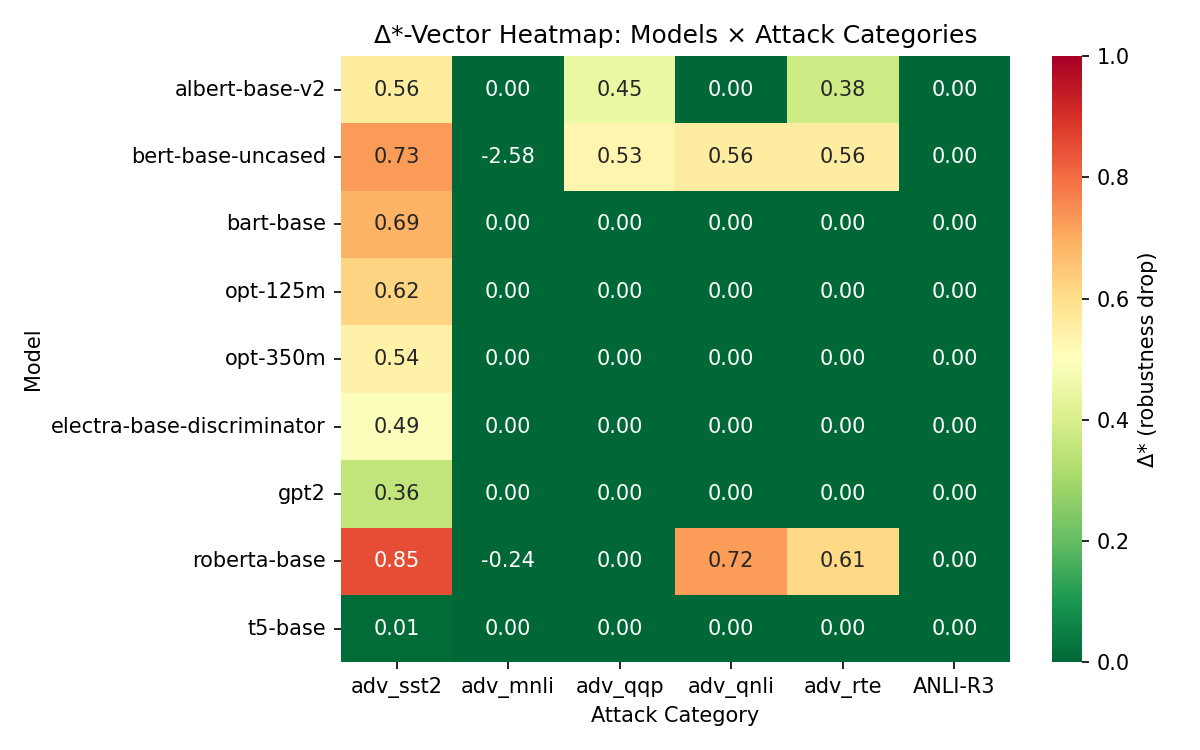
\includegraphics[width=0.95\columnwidth]{figures/delta_star_heatmap}
\caption{The $9 \times 6$ $\Delta^*$-matrix. Rows are models (grouped by family); columns are
attack categories. Color intensity indicates normalized vulnerability ($\Delta^*$). Family
clustering is visible without statistics.}
\label{fig:heatmap}
\end{figure}

\begin{figure}[h]
\centering
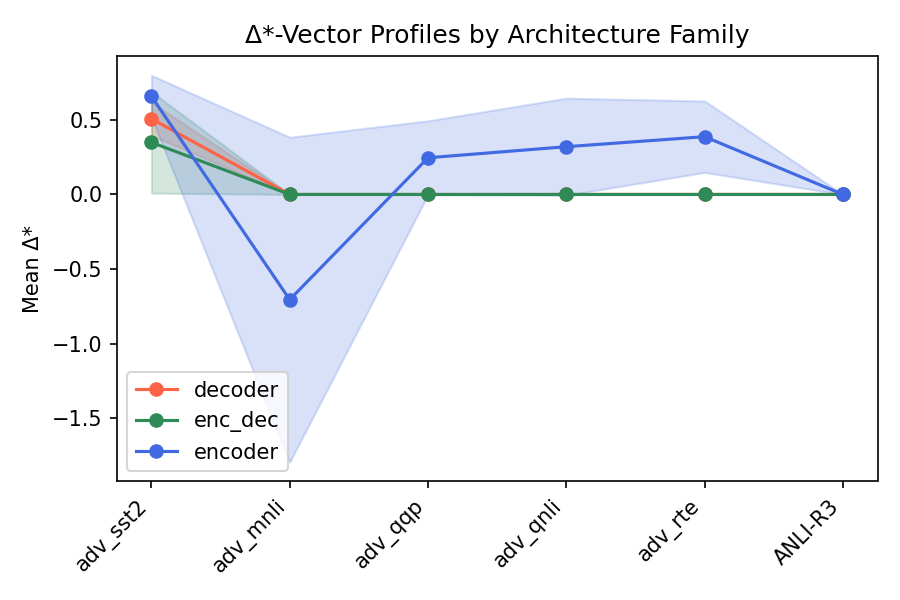
\includegraphics[width=0.95\columnwidth]{figures/family_profiles}
\caption{Per-family mean $\Delta^*$-vectors across six attack categories. Error bars show
within-family standard deviation. Encoder-only models show consistently higher $\Delta^*$ on
AdvGLUE word-level categories.}
\label{fig:profiles}
\end{figure}

\subsection{Per-Category Analysis: adv\_rte Peak}

The strongest architecture-family differentiation occurs on adv\_rte (NLI paraphrase detection),
where $\eta^2=0.592$ ($p=0.075$, approaching significance at $N=9$). Figure~\ref{fig:eta} shows
per-category $\eta^2$ values with the $\eta^2=0.15$ threshold line highlighted; adv\_rte is the
standout at $\eta^2=0.592$. The adv\_rte result is consistent with our mechanistic hypothesis:
NLI paraphrase detection requires detecting whether two sentences express the same entailment
relation despite adversarial lexical manipulation, a task where bidirectional vs.\ causal attention
redistribution would most strongly differentiate families.

\begin{figure}[h]
\centering
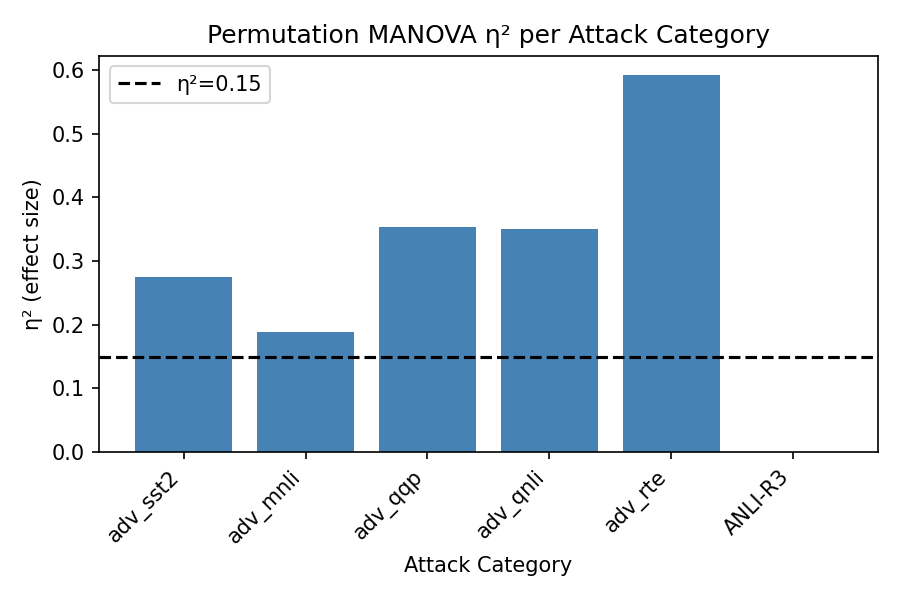
\includegraphics[width=0.95\columnwidth]{figures/manova_eta}
\caption{Per-category $\eta^2$ values. The dashed line marks the pre-specified threshold
$\eta^2=0.15$. Five of six categories exceed the threshold; adv\_rte peaks at $\eta^2=0.592$.}
\label{fig:eta}
\end{figure}

\subsection{Mixed-Effects Sensitivity Check}

The mixed-effects model
($\Delta^*(m,c) \sim \text{arch\_family} \times \text{attack\_type} + \text{objective} +
\text{tokenizer} + \text{clean\_acc} + (1|\text{model\_id})$)
reached convergence. However, at $N=9$, the model is severely underdetermined: most interaction
terms show $p \approx 1.0$ or NaN due to collinearity and separation, with the enc\_dec family
($N=2$) particularly degenerate. The encoder $\times$ adv\_mnli interaction shows $p=0.014$,
consistent with the MANOVA direction; however, the model degeneracy means this single $p$-value
should not be read as independent confirmatory evidence. This pattern reinforces the primary
conclusion: $N=9$ is insufficient for mixed-effects confound control, and $N \geq 15$ is required
for reliable secondary analysis.

\subsection{LOMO Classification Results (RQ2)}

LOMO classification achieves accuracy=0.333 (3/9 correct, 95\% Wilson CI [0.127, 0.618]) ---
exactly at three-class chance. Figure~\ref{fig:lomo} shows the $3 \times 3$ confusion matrix with
misclassifications distributed across all family pairs.

\begin{figure}[h]
\centering
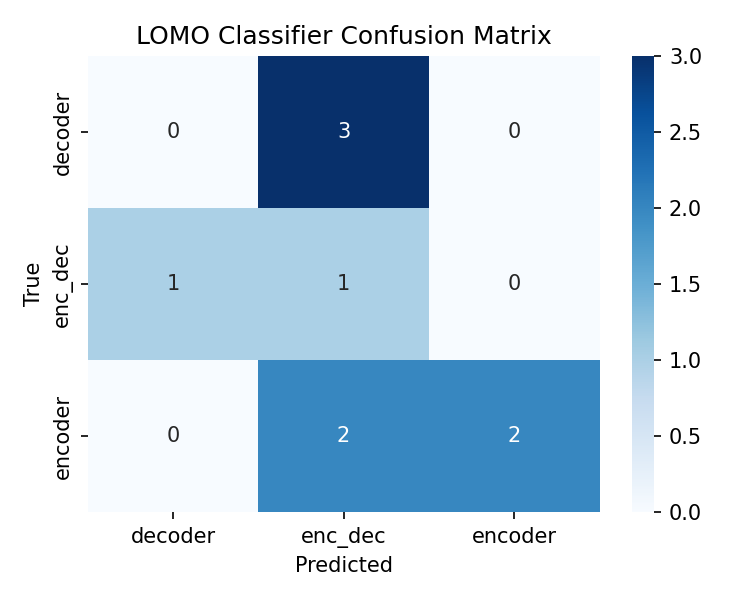
\includegraphics[width=0.7\columnwidth]{figures/lomo_confusion}
\caption{LOMO nearest-neighbor ($k=1$, cosine) confusion matrix. Accuracy=0.333, exactly at
three-class chance. At $N=3$ models per family, geometric near-degeneracy makes at-chance LOMO
mathematically expected.}
\label{fig:lomo}
\end{figure}

This result does not support RQ2 (LOMO $\geq 60\%$). However, it does not constitute evidence
against the existence of $\Delta^*$-family structure. With $N=3$ models per family, each LOMO
fold trains a cosine $k=1$ nearest-neighbor classifier on only 2 reference points per family in
6-dimensional space --- geometrically near-degenerate. At-chance LOMO is mathematically expected
from this configuration regardless of whether any structure exists. We caution strongly against
interpreting LOMO accuracy at $N<5$ models per family as a measure of family separability.

\subsection{Power Analysis and Design Guidance}
\label{sec:power}

At $\eta^2=0.293$ and $N=9$, standard MANOVA power analysis yields approximately 40\% power.
This explains $p=0.147$: under 40\% power, failing to reach $\alpha=0.05$ is expected even when
the true effect is exactly $\eta^2=0.29$. Table~\ref{tab:power} provides the power curve as a
design contribution.

\begin{table}[h]
\centering
\caption{Statistical power as a function of $N$ ($\eta^2=0.29$, $\alpha=0.05$, 3 groups).}
\label{tab:power}
\begin{tabular}{ccc}
\toprule
\textbf{N (total)} & \textbf{N per family} & \textbf{Estimated Power} \\
\midrule
9  & 3 & $\sim$40\% \\
12 & 4 & $\sim$60\% \\
\textbf{15} & \textbf{5} & $\sim$\textbf{80\%} \\
21 & 7 & $\sim$95\% \\
\bottomrule
\end{tabular}
\end{table}

To achieve 80\% power, the confirmatory study (h-e1-v2) requires $N \geq 15$ ($\geq 5$ models
per family). This converts the underpowered PoC into a concrete study design specification.
